\chapter{模型推断与平均}

% ============ §8.1 引言 ============
\section{引言}

此前章节中，模型拟合（学习）通过最小化平方和（回归）或交叉熵（分类）来实现。这些最小化本质上都是最大似然估计的特例。

本章将系统介绍最大似然方法和贝叶斯推断方法，并讨论 Bootstrap 在这两种框架下的角色。最后介绍模型平均与改进的相关技术，包括委员会方法、Bagging、Stacking 和 Bumping。

% ============ §8.2 Bootstrap 与最大似然方法 ============
\section{Bootstrap 与最大似然方法}

\subsection{一个光滑示例}

Bootstrap 提供了一种直接的计算方式，通过从训练数据中抽样来评估不确定性。这里以一个一维光滑问题为例，展示其与最大似然的联系。

\textbf{数据与模型：} 训练数据 $\mathbf{Z} = \{z_1, \ldots, z_N\}$，$z_i = (x_i, y_i)$，$x_i$ 为一维输入，$y_i$ 为响应。考虑 $N=50$ 的数据点（图 8.1 左面板）。用三次样条拟合，在 $X$ 的四分位处放置三个结点，构成 7 维 B-样条基函数空间（图 8.1 右面板）：

\begin{figure}[ht]
    \centering
    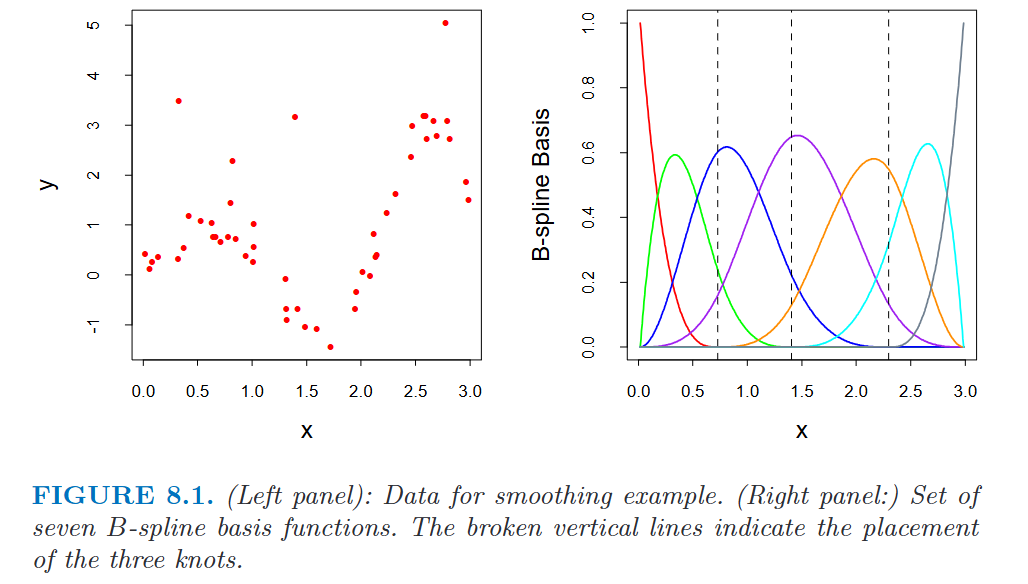
\includegraphics[width=0.9\textwidth]{Chapters/pic/ch_模型推断与平均/figure_8_1.png}
    \caption{（左）光滑示例的数据。（右）七个 B-样条基函数。竖直虚线指示三个结点的位置。}
    \label{fig:8_1}
\end{figure}
\begin{equation}\label{eq:8_1}
    \mu(x) = \sum_{j=1}^{7} \beta_j h_j(x)
\end{equation}
令 $\mathbf{H}$ 为 $N \times 7$ 矩阵，$h_{ij} = h_j(x_i)$。最小二乘估计为：
\begin{equation}\label{eq:8_2}
    \hat{\bm{\beta}} = (\mathbf{H}^T\mathbf{H})^{-1}\mathbf{H}^T\mathbf{y}
\end{equation}

$\hat{\bm{\beta}}$ 的估计协方差矩阵为：
\begin{equation}\label{eq:8_3}
    \widehat{\mathrm{Var}}(\hat{\bm{\beta}}) = (\mathbf{H}^T\mathbf{H})^{-1}\hat{\sigma}^2
\end{equation}
其中 $\hat{\sigma}^2 = \sum_{i=1}^{N}(y_i - \hat{\mu}(x_i))^2/N$。预测 $\hat{\mu}(x) = \mathbf{h}(x)^T\hat{\bm{\beta}}$ 的标准误差为：
\begin{equation}\label{eq:8_4}
    \widehat{\mathrm{se}}[\hat{\mu}(x)] = [\mathbf{h}(x)^T(\mathbf{H}^T\mathbf{H})^{-1}\mathbf{h}(x)]^{1/2}\,\hat{\sigma}
\end{equation}

\begin{figure}
    \centering
    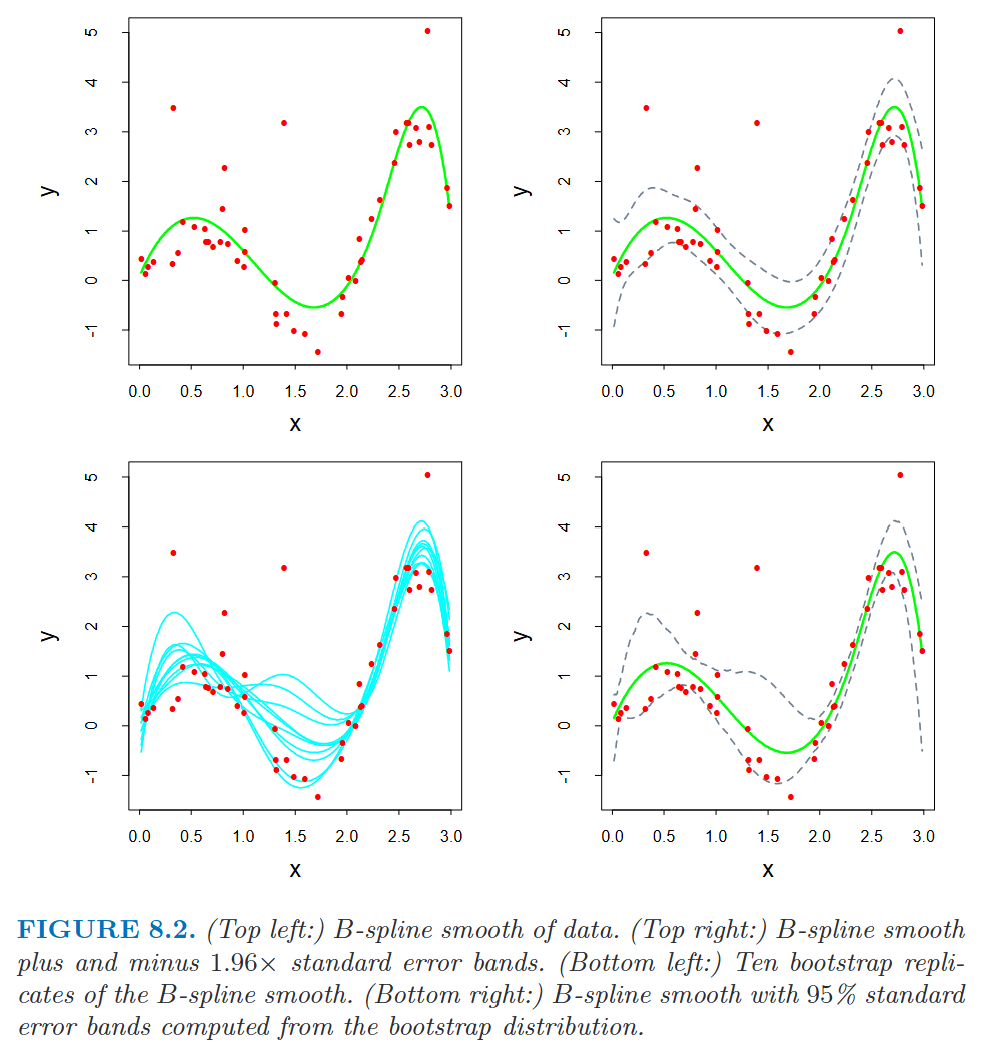
\includegraphics[width=0.9\textwidth]{Chapters/pic/ch_模型推断与平均/figure_8_2.png}
    \caption{（左上）数据的 B-样条光滑。（右上）B-样条光滑 $\pm 1.96\times$ 标准误差带。（左下）B-样条光滑的 10 次 Bootstrap 重复。（右下）由 Bootstrap 分布构造的 95\% 标准误差带。}
    \label{fig:8_2}
\end{figure}

右上展示了 $\hat{\mu}(x) \pm 1.96\cdot\widehat{\mathrm{se}}$ 的逐点 95\% 置信带。

\textbf{Bootstrap 做法：} 从训练数据中有放回地抽取 $B$ 个大小为 $N=50$ 的数据集，抽样单位为 $(x_i, y_i)$ 对。对每个 Bootstrap 数据集拟合三次样条 $\hat{\mu}^*(x)$。图 8.2 左下展示了 10 次 Bootstrap 光滑，右下为由 $B=200$ 次 Bootstrap 的分位数构造的 95\% 置信带——与最小二乘置信带相似，在端点处略宽。

\subsection{非参数 Bootstrap 与参数 Bootstrap}

上述直接从数据中有放回重抽样的做法称为\textbf{非参数 Bootstrap}（nonparametric bootstrap），它是「无模型」的——只用原始数据本身生成新数据集，不依赖特定的参数模型。

若假设模型误差为高斯:
\begin{equation}\label{eq:8_5}
    Y = \mu(X) + \varepsilon,\quad \varepsilon \sim N(0, \sigma^2),\quad \mu(x) = \sum_{j=1}^{7}\beta_j h_j(x)
\end{equation}
则可使用\textbf{参数 Bootstrap}（parametric bootstrap）：向拟合值添加高斯噪声模拟新响应
\begin{equation}\label{eq:8_6}
    y_i^* = \hat{\mu}(x_i) + \varepsilon_i^*,\quad \varepsilon_i^* \sim N(0, \hat{\sigma}^2),\quad i=1,\ldots,N
\end{equation}
重复 $B$ 次，重新拟合 B-样条光滑。参数 Bootstrap 给出的置信带与最小二乘置信带\textbf{精确一致}——因为高斯误差的可加性。

\subsection{最大似然推断}

\subsubsection{基本定义}

设观测的密度函数（或概率质量函数）为 $z_i \sim g_\theta(z)$，其中 $\theta$ 为未知参数。似然函数定义为：
\begin{equation}\label{eq:likelihood}
    L(\theta; \mathbf{Z}) = \prod_{i=1}^{N} g_\theta(z_i)
\end{equation}

对数似然（log-likelihood）为：
\begin{equation}\label{eq:loglik}
    \ell(\theta; \mathbf{Z}) = \sum_{i=1}^{N} \log g_\theta(z_i) = \sum_{i=1}^{N} \ell(\theta; z_i)
\end{equation}
最大似然估计（MLE）$\hat{\theta}$ 使 $\ell(\theta; \mathbf{Z})$ 最大化。

\textbf{得分函数（score function）：}
\begin{equation}\label{eq:score}
    \dot{\ell}(\theta; \mathbf{Z}) = \sum_{i=1}^{N} \dot{\ell}(\theta; z_i),\quad \dot{\ell}(\theta; z_i) = \frac{\partial \ell(\theta; z_i)}{\partial\theta}
\end{equation}

\textbf{信息矩阵（information matrix）：}
\begin{equation}\label{eq:info}
    \mathbf{I}(\theta) = -\sum_{i=1}^{N} \frac{\partial^2 \ell(\theta; z_i)}{\partial\theta\,\partial\theta^T}
\end{equation}
在 $\hat{\theta}$ 处取值时称为\textbf{观测信息}（observed information）。\textbf{Fisher 信息}（期望信息）为 $\mathbf{i}(\theta) = \E_\theta[\mathbf{I}(\theta)]$。

MLE 属于\textbf{频率学派}框架：参数 $\theta$ 是固定但未知的常数，数据是随机的；推断依赖「重复抽样下估计量的行为」。与之对照，\textbf{贝叶斯学派}将 $\theta$ 视为随机变量，用先验 $\Pr(\theta)$ 表达初始不确定性，数据固定后通过贝叶斯公式更新为后验 $\Pr(\theta\mid\mathbf{Z})$。频率学派给出置信区间（「若重复实验，95\% 的区间会覆盖 $\theta$」），贝叶斯给出可信区间（「$\theta$ 有 95\% 概率在此区间」）。

\textbf{实践中真的知道分布族吗？} 常不知道确切形式，但有合理理由假设：计数数据 → Poisson，二元结果 → Bernoulli，大样本独立和 → 近似正态（CLT）。有时为了数学可行性而假设（如回归中的高斯误差）。当不愿假设分布时，\textbf{非参数 Bootstrap} 是替代方案——直接从数据重抽样，不指定 $g_\theta$。这也是 §8.2 将 Bootstrap 和 MLE 放在同一章的原因。

\subsubsection{MLE 框架的完整定义体系}

除已给出的基本定义外，MLE 框架还包括以下核心概念：

\begin{itemize}
    \item \textbf{一致性（Consistency）：} $\hat{\theta} \xrightarrow{P} \theta_0$（$N\to\infty$），样本越大估计越准。
    \item \textbf{渐近有效性（Asymptotic efficiency）：} $N\to\infty$ 时 MLE 达到 Cramér-Rao 下界（见下文详述），在所有渐近无偏估计中方差最小。
    \item \textbf{不变性（Invariance）：} 若 $\hat{\theta}$ 是 $\theta$ 的 MLE，则 $g(\hat{\theta})$ 是 $g(\theta)$ 的 MLE。
    \item \textbf{Delta 方法：} 用于求 $g(\hat{\theta})$ 的渐近分布：$\sqrt{N}(g(\hat{\theta}) - g(\theta_0)) \xrightarrow{d} N(0, g'(\theta_0)^2/\mathbf{i}(\theta_0))$。
    \item \textbf{似然比检验（LRT）：} $2[\ell(\hat{\theta}) - \ell(\theta_0)] \xrightarrow{d} \chi^2_p$，即式 \eqref{eq:chisq}。
    \item \textbf{Wald 检验：} 直接用 $\hat{\theta}$ 的渐近正态性检验 $H_0: \theta=\theta_0$。
    \item \textbf{得分检验（Rao）：} 仅需在原假设下拟合模型，计算量最小。
    \item \textbf{剖面似然（Profile likelihood）：} 处理多余参数——对不感兴趣的参数取最大化后留轮廓。
    \item \textbf{指数族：} GLM 的基础，似然标准形式为 $\exp\{[y\theta - b(\theta)]/a(\phi) + c(y,\phi)\}$。
\end{itemize}

LRT、Wald、得分检验合称 MLE 框架的「三大检验」。

\begin{figure}[H]
    \centering
    \begin{tikzpicture}[
        node distance=0.7cm and 1.4cm,
        core/.style={draw, rounded corners, fill=blue!8, text width=3cm, align=center, minimum height=0.8cm, font=\small\bfseries},
        defbox/.style={draw, rounded corners, fill=gray!8, text width=2.8cm, align=center, minimum height=0.7cm, font=\footnotesize},
        propbox/.style={draw, rounded corners, fill=green!6, text width=3.2cm, align=center, minimum height=0.7cm, font=\footnotesize},
        testbox/.style={draw, rounded corners, fill=orange!8, text width=2.6cm, align=center, minimum height=0.7cm, font=\footnotesize},
        arrow/.style={->, >=stealth, thick},
        dasharrow/.style={->, >=stealth, dashed, thick, gray}
    ]
    % Row 1: Data + Model → Core
    \node[defbox] (data) {数据 $\mathbf{Z}=(z_1,\ldots,z_N)$\\iid 抽样};
    \node[defbox, left=of data] (model) {参数模型 $g_\theta(z)$\\指定分布族};
    \node[core, left=of model, text width=3.5cm] (like) {似然函数\\$L(\theta)=\prod_i g_\theta(z_i)$};

    \draw[arrow] (data) -- (model);
    \draw[arrow] (model) -- (like);

    % Row 2: log-lik → score → MLE
    \node[core, below=of like] (loglik) {对数似然 $\ell(\theta)=\sum\log g_\theta(z_i)$};
    \node[core, right=of loglik] (score) {得分函数 $\dot{\ell}(\theta)$\\$\E[\dot{\ell}]=0$};
    \node[core, right=of score] (mle) {\textbf{MLE $\hat{\theta}$}\\$\dot{\ell}(\hat{\theta})=0$};

    \draw[arrow] (like) -- (loglik);
    \draw[arrow] (loglik) -- (score);
    \draw[arrow] (score) -- (mle);

    % Row 3: Information → Inference
    \node[defbox, below=of loglik] (info) {信息矩阵 $\mathbf{I}(\theta)$\\$=-\sum\partial^2\ell/\partial\theta^2$};
    \node[defbox, right=of info] (fish) {Fisher 信息 $\mathbf{i}(\theta)$\\$=\E[\mathbf{I}(\theta)]$};
    \node[defbox, right=of fish] (se) {标准误差\\$\widehat{\mathrm{se}}=\sqrt{\mathbf{I}^{-1}_{jj}}$};
    \node[core, right=of se] (ci) {置信区间\\$\hat{\theta}\pm z\cdot\widehat{\mathrm{se}}$};

    \draw[arrow] (loglik) -- (info);
    \draw[arrow] (info) -- (fish);
    \draw[arrow] (fish) -- (se);
    \draw[arrow] (se) -- (ci);

    % Row 4: Properties
    \node[propbox, below=of info, text width=3.5cm] (cons) {\textbf{一致性}\\$\hat{\theta}\xrightarrow{P}\theta_0$};
    \node[propbox, right=0.15cm of cons, text width=3.2cm] (eff) {\textbf{渐近有效性}\\达到 CRLB};
    \node[propbox, right=0.15cm of eff, text width=3.2cm] (asym) {\textbf{渐近正态}\\$\hat{\theta}\stackrel{\cdot}{\sim}N(\theta_0,\mathbf{i}^{-1})$};
    \node[propbox, right=0.15cm of asym, text width=3.2cm] (inv) {\textbf{不变性}\\$g(\hat{\theta})$ 是 $g(\theta)$ 的 MLE};

    \draw[dasharrow] (mle.south) -- (cons.north);
    \draw[dasharrow] (mle.south) -- (eff.north);
    \draw[dasharrow] (mle.south) -- (asym.north);
    \draw[dasharrow] (mle.south) -- (inv.north);

    % Row 5: Three Tests
    \node[testbox, below=1.2cm of cons, xshift=-1.6cm] (lrt) {\textbf{似然比 LRT}\\$2[\ell(\hat{\theta})-\ell(\theta_0)]\sim\chi^2$};
    \node[testbox, right=0.15cm of lrt] (wald) {\textbf{Wald 检验}\\用渐近正态性};
    \node[testbox, right=0.15cm of wald] (rao) {\textbf{得分检验}\\仅需 $H_0$ 下拟合};

    \draw[dasharrow] (ci.south) -- (lrt.north);
    \draw[dasharrow] (ci.south) -- (wald.north);
    \draw[dasharrow] (ci.south) -- (rao.north);

    % Row 6: Additional Tools
    \node[defbox, below=1cm of lrt, xshift=1cm, text width=3cm] (delta) {Delta 方法\\$g(\hat{\theta})$ 的渐近分布};
    \node[defbox, right=0.15cm of delta, text width=3cm] (prof) {剖面似然\\处理多余参数};
    \node[defbox, right=0.15cm of prof, text width=3cm] (expfam) {指数族\\GLM 的基础};

    \end{tikzpicture}
    \caption{MLE 框架的完整定义体系。自上而下：数据+模型 → 似然 → 对数似然 → 得分 → MLE；左下：大样本性质（一致性、有效性、渐近正态、不变性）；右下：三大检验（LRT、Wald、得分）；底部：扩展工具（Delta 方法、剖面似然、指数族）。}
    \label{fig:MLE_framework}
\end{figure}

\subsubsection{Cramér-Rao 下界}

Cramér-Rao 下界（CRLB）给出了\textbf{所有无偏估计量方差的下限}，是 Fisher 信息最核心的应用。设 $T(\mathbf{Z})$ 是 $\theta$ 的任意无偏估计量（$\E_\theta[T] = \theta$），在正则条件下：
\begin{equation}\label{eq:CRLB}
    \Var_\theta(T) \geq \frac{1}{\mathbf{i}(\theta)}
\end{equation}
其中 $\mathbf{i}(\theta) = \E_\theta[(\frac{\partial}{\partial\theta}\log g_\theta(Z))^2]$ 是 Fisher 信息（单参数情形）。

\textbf{多参数推广：} 对 $\bm{\theta} \in \mathbb{R}^p$，无偏估计量 $\mathbf{T}$ 的协方差矩阵满足 $\mathrm{Cov}_\theta(\mathbf{T}) \succeq \mathbf{i}(\bm{\theta})^{-1}$（矩阵差为半正定），各分量方差 $\Var_\theta(T_j) \geq [\mathbf{i}(\bm{\theta})^{-1}]_{jj}$。

\textbf{三种理解角度：}
\begin{enumerate}
    \item \textbf{参数估计精度的理论上限} — $\mathbf{i}(\theta)$ 越大，CRLB 越低，参数能被估计得越精确。MLE 渐近达到此下界（渐近有效性），这就是为什么 MLE 在理论上是最优的。
    \item \textbf{得分函数的方差（基础定义）} — $\mathbf{i}(\theta) = \Var_\theta[\dot{\ell}(\theta; Z)]$。得分函数衡量「数据对参数的敏感度」：数据轻微变化，得分剧烈波动 → 方差大 → 信息多 → 下界低。若不管数据怎么变得分几乎不动 → 信息少 → 参数难以估计。
    \item \textbf{区分邻近参数的能力（KL 散度视角）} — 两个邻近参数 $\theta$ 和 $\theta+d\theta$ 对应分布的 KL 散度展开为 $\mathrm{KL}(g_\theta \parallel g_{\theta+d\theta}) \approx \frac{1}{2}\mathbf{i}(\theta)(d\theta)^2$。Fisher 信息大 → 邻近参数对应分布差异大 → 容易区分 → 可精确估计。Fisher 信息小 → 参数变化几乎不影响分布 → 不可识别。
\end{enumerate}

\textbf{与观测信息的区别：} 观测信息 $\mathbf{I}(\hat{\theta})$ 和 Fisher 信息 $\mathbf{i}(\hat{\theta})$ 在大样本下等价，均可用于构造标准误差。实践中 $\mathbf{I}(\hat{\theta})$ 更常用——它只需在 MLE 处计算二阶导数，无需对 $g_\theta$ 积分。

\subsubsection{正则条件与推导}

CRLB 的成立需要以下\textbf{正则条件（regularity conditions）}：

\begin{enumerate}
    \item \textbf{支撑集与 $\theta$ 无关：} $\{z: g_\theta(z) > 0\}$ 不依赖于 $\theta$。这排除了均匀分布 $U(0,\theta)$ 等边界随参数移动的情形。
    \item \textbf{可微性：} $g_\theta(z)$ 对 $\theta$ 可微，且积分和求导可交换次序：
    \begin{equation}
        \frac{\partial}{\partial\theta}\int g_\theta(z)\,dz = \int \frac{\partial}{\partial\theta}g_\theta(z)\,dz = 0
    \end{equation}
    \item \textbf{得分函数零均值：} 由条件 2 立即得到 $\E_\theta[\dot{\ell}(\theta; Z)] = 0$。
    \item \textbf{Fisher 信息有限且正定：} $0 < \mathbf{i}(\theta) < \infty$。
\end{enumerate}

\textbf{推导（单参数情形）：} 设 $T = T(\mathbf{Z})$ 为 $\theta$ 的任意无偏估计量，$\E_\theta[T] = \theta$。

由无偏性 $\int T(\mathbf{z})\,g_\theta(\mathbf{z})\,d\mathbf{z} = \theta$，两边对 $\theta$ 求导：
\begin{equation}\label{eq:cr_deriv1}
    \int T(\mathbf{z})\,\frac{\partial g_\theta(\mathbf{z})}{\partial\theta}\,d\mathbf{z} = 1
\end{equation}

利用 $\frac{\partial g_\theta}{\partial\theta} = g_\theta \cdot \frac{\partial\log g_\theta}{\partial\theta} = g_\theta \cdot \dot{\ell}(\theta)$，代入得：
\begin{equation}\label{eq:cr_deriv2}
    \int T(\mathbf{z})\,\dot{\ell}(\theta; \mathbf{z})\,g_\theta(\mathbf{z})\,d\mathbf{z} = \E_\theta[T\cdot\dot{\ell}] = 1
\end{equation}

又 $\E_\theta[\dot{\ell}] = 0$，故 $\Cov_\theta(T, \dot{\ell}) = \E_\theta[T\cdot\dot{\ell}] - \E_\theta[T]\cdot\E_\theta[\dot{\ell}] = 1$。

由 Cauchy-Schwarz 不等式：
\begin{equation}\label{eq:cr_deriv3}
    1 = \Cov_\theta(T, \dot{\ell})^2 \leq \Var_\theta(T)\cdot\Var_\theta(\dot{\ell}) = \Var_\theta(T)\cdot\mathbf{i}(\theta)
\end{equation}

移项即得：
\begin{equation}\label{eq:cr_deriv4}
    \boxed{\Var_\theta(T) \geq \frac{1}{\mathbf{i}(\theta)}}
\end{equation}

\textbf{取等条件：} 当且仅当 $T$ 和 $\dot{\ell}$ 线性相关，即 $\dot{\ell}(\theta) = a(\theta)(T - \theta)$ 时等号成立。这意味着分布族必须是指数族且 $T$ 是充分统计量——这正是 MLE 渐近达到下界的深层原因。

\textbf{直观小结：} CRLB 的推导核心只有三步：无偏性 → 协方差为 1 → Cauchy-Schwarz 放缩。Fisher 信息出现在分母是因为它恰好是得分函数的方差。

\subsubsection{三个完整示例}

\textbf{例 1：Bernoulli 试验（$p$ 未知）。}
$N$ 次独立抛硬币，观测 $y_i \in \{0,1\}$，$Y_i \sim \mathrm{Bernoulli}(p)$。

\begin{itemize}
    \item \textbf{模型：} $g_p(y) = p^y(1-p)^{1-y}$
    \item \textbf{对数似然：} $\ell(p) = \sum y_i \log p + \sum(1-y_i)\log(1-p) = N\bar{y}\log p + N(1-\bar{y})\log(1-p)$
    \item \textbf{得分（找 MLE）：} $\dot{\ell}(p) = \frac{N\bar{y}}{p} - \frac{N(1-\bar{y})}{1-p} = 0 \;\Rightarrow\; \hat{p} = \bar{y}$（样本均值）
    \item \textbf{信息（算 SE）：} $\mathbf{I}(\hat{p}) = -\ddot{\ell}(\hat{p}) = \frac{N}{\hat{p}(1-\hat{p})}$，故 $\widehat{\mathrm{se}}(\hat{p}) = \sqrt{\hat{p}(1-\hat{p})/N}$
    \item \textbf{CI（表达不确定性）：} $\hat{p} \pm 1.96\sqrt{\frac{\hat{p}(1-\hat{p})}{N}}$
\end{itemize}

\textbf{数值演示：} $N=100$ 次抛硬币，58 次正面。

\begin{itemize}
    \item \textbf{MLE：} $\hat{p} = 58/100 = 0.58$
    \item \textbf{SE：} $\widehat{\mathrm{se}} = \sqrt{0.58\times0.42/100} = 0.049$
    \item \textbf{95\% CI：} $0.58 \pm 1.96\times 0.049 = [0.484,\; 0.676]$
\end{itemize}

\textbf{结论：} 硬币正面概率的 MLE 为 0.58，标准误差 0.049（基于 100 次观测的信息量）。95\% 置信区间 [0.484, 0.676] 包含 0.5——因此 58 次正面并不构成硬币不公平的充分证据（在 95\% 置信水平下不能拒绝 $p=0.5$）。这里得分求出了点估计，信息量化了精度（SE=0.049 意味着要检测出 0.08 的偏差，大约需要 $1.96\times0.049<0.08\to N$ 不足），CI 把精度翻译为可读的区间。

\textbf{例 2：高斯分布（$\mu$ 未知，$\sigma^2$ 已知）。}
$Y_i \stackrel{\text{iid}}{\sim} N(\mu, \sigma_0^2)$，$\sigma_0^2$ 已知。

\begin{itemize}
    \item \textbf{对数似然：} $\ell(\mu) = -\frac{N}{2}\log(2\pi\sigma_0^2) - \frac{1}{2\sigma_0^2}\sum(y_i - \mu)^2$
    \item \textbf{得分（找 MLE）：} $\dot{\ell}(\mu) = \frac{1}{\sigma_0^2}\sum(y_i - \mu) = 0 \;\Rightarrow\; \hat{\mu} = \bar{y}$
    \item \textbf{Fisher 信息（算 SE）：} $\mathbf{i}(\mu) = -\E[\ddot{\ell}(\mu)] = N/\sigma_0^2$，$\widehat{\mathrm{se}}(\hat{\mu}) = \sigma_0/\sqrt{N}$
    \item \textbf{CI（表达不确定性）：} $\bar{y} \pm 1.96\,\sigma_0/\sqrt{N}$
\end{itemize}

\textbf{数值演示：} 测量某零件长度 25 次，已知仪器精度 $\sigma_0=0.2$ mm，$\bar{y}=10.3$ mm。

\begin{itemize}
    \item \textbf{MLE：} $\hat{\mu} = 10.3$
    \item \textbf{SE：} $\widehat{\mathrm{se}} = 0.2/\sqrt{25} = 0.04$
    \item \textbf{95\% CI：} $10.3 \pm 1.96\times 0.04 = [10.22,\; 10.38]$
\end{itemize}

\textbf{结论：} 零件平均长度为 10.3 mm，标准误差 0.04 mm（25 次测量 + 已知精度提供了足够信息）。95\% CI [10.22, 10.38] 很窄，说明估计相当精确。如果规格要求为 10.0 mm，则 CI 不包含 10.0——有明显偏差。这里 $\sigma_0$ 已知使得信息可以直接写为 $N/\sigma_0^2$，不需要从数据估计。

\textbf{例 3：高斯分布（$\mu$ 和 $\sigma^2$ 均未知）。}
$Y_i \stackrel{\text{iid}}{\sim} N(\mu, \sigma^2)$，$\theta = (\mu, \sigma^2)$。

\begin{itemize}
    \item \textbf{对数似然：} $\ell(\mu,\sigma^2) = -\frac{N}{2}\log\sigma^2 - \frac{1}{2\sigma^2}\sum(y_i - \mu)^2$（略去常数项）
    \item \textbf{得分方程组（联合求解）：}
    $\frac{\partial\ell}{\partial\mu} = \frac{1}{\sigma^2}\sum(y_i - \mu) = 0$，
    $\frac{\partial\ell}{\partial\sigma^2} = -\frac{N}{2\sigma^2} + \frac{1}{2\sigma^4}\sum(y_i - \mu)^2 = 0$
    \item \textbf{MLE：} $\hat{\mu} = \bar{y}$，$\hat{\sigma}^2 = \frac{1}{N}\sum(y_i - \bar{y})^2$（分母为 $N$，非 $N-1$——MLE 不校正自由度）
    \item \textbf{观测信息矩阵：} 块对角（$\mu$ 和 $\sigma^2$ 在 MLE 处信息正交），
    $\mathbf{I}_{11} = N/\hat{\sigma}^2$，$\mathbf{I}_{22} = N/(2\hat{\sigma}^4)$
    \item \textbf{SE：} $\widehat{\mathrm{se}}(\hat{\mu}) = \hat{\sigma}/\sqrt{N}$，$\widehat{\mathrm{se}}(\hat{\sigma}^2) = \hat{\sigma}^2\sqrt{2/N}$
    \item \textbf{CI for $\mu$：} 由于 $\sigma^2$ 未知，实际用 $t$ 分布：$\bar{y} \pm t_{N-1, 0.975}\cdot s/\sqrt{N}$（$s$ 为样本标准差 $s^2 = \sum(y_i-\bar{y})^2/(N-1)$）；大样本下近似于 $\bar{y} \pm 1.96\cdot\hat{\sigma}/\sqrt{N}$
\end{itemize}

\textbf{数值演示：} 测量 16 次，$\bar{y}=10.3$，$s=0.5$，$\hat{\sigma}=0.484$。

\begin{itemize}
    \item \textbf{MLE：} $\hat{\mu}=10.3$，$\hat{\sigma}^2=0.234$
    \item \textbf{SE：} $\widehat{\mathrm{se}}(\hat{\mu}) = 0.484/\sqrt{16}=0.121$，$\widehat{\mathrm{se}}(\hat{\sigma}^2)=0.234\times\sqrt{2/16}=0.083$
    \item \textbf{95\% CI for $\mu$：} $10.3 \pm 2.131\times 0.125 = [10.03,\; 10.57]$（用 $t_{15,0.975}=2.131$ 和 $s/\sqrt{16}=0.125$）；大样本近似：$10.3 \pm 1.96\times 0.121 = [10.06,\; 10.54]$
    \item \textbf{95\% CI for $\sigma^2$：} 基于卡方近似 $[\hat{\sigma}^2\cdot\chi^2_{15,0.025}/15,\; \hat{\sigma}^2\cdot\chi^2_{15,0.975}/15] = [0.128,\; 0.519]$
\end{itemize}

\textbf{结论：} 当 $\sigma^2$ 未知时，$\mu$ 的 SE 变大了（0.121 vs 例 2 的 0.04）——多估计一个参数消耗了信息。信息矩阵的块对角性意味着 $\mu$ 和 $\sigma^2$ 的 MLE 渐近不相关，可以分别推断。$\hat{\sigma}^2$ 的 MLE 有有限样本偏差（$\E[\hat{\sigma}^2] = \frac{15}{16}\sigma^2$），但 $N=16$ 时偏差已很小，且渐近性质优良——这是 MLE 的典型特征。

\subsubsection{渐近正态性}

经典结果：当 $N \to \infty$ 时，MLE 的抽样分布趋于正态：
\begin{equation}\label{eq:asym_normal}
    \hat{\theta} \to N\bigl(\theta_0, \mathbf{i}(\theta_0)^{-1}\bigr)
\end{equation}
其中 $\theta_0$ 为真实参数值。实践中用以下近似：
\begin{equation}\label{eq:MLE_approx}
    \hat{\theta} \stackrel{\cdot}{\sim} N\bigl(\hat{\theta}, \mathbf{i}(\hat{\theta})^{-1}\bigr) \;\text{或}\; N\bigl(\hat{\theta}, \mathbf{I}(\hat{\theta})^{-1}\bigr)
\end{equation}

标准误差的估计为 $\sqrt{\mathbf{i}(\hat{\theta})^{-1}_{jj}}$ 或 $\sqrt{\mathbf{I}(\hat{\theta})^{-1}_{jj}}$。置信区间形如 $\hat{\theta}_j \pm z^{(1-\alpha)}\cdot\widehat{\mathrm{se}}$。

也可直接利用似然函数构造更精确的置信区域——利用卡方近似：
\begin{equation}\label{eq:chisq}
    2[\ell(\hat{\theta}) - \ell(\theta_0)] \sim \chi^2_p
\end{equation}

\subsubsection{光滑示例的最大似然解}

在光滑示例中，$\theta = (\bm{\beta}, \sigma^2)$，对数似然为：
\begin{equation}\label{eq:8_20}
    \ell(\theta) = -\frac{N}{2}\log\sigma^2 2\pi - \frac{1}{2\sigma^2}\sum_{i=1}^{N}\bigl(y_i - \mathbf{h}(x_i)^T\bm{\beta}\bigr)^2
\end{equation}
MLE 解与最小二乘一致，$\bm{\beta}$ 的信息矩阵块为 $\mathbf{I}(\bm{\beta}) = \mathbf{H}^T\mathbf{H}/\sigma^2$，方差估计 $\widehat{\mathrm{Var}}(\hat{\bm{\beta}}) = (\mathbf{H}^T\mathbf{H})^{-1}\hat{\sigma}^2$ 与 (8.3) 一致。

\subsection{Bootstrap 与最大似然的比较}

Bootstrap 本质上是\textbf{非参数或参数最大似然的计算机实现}。其优势在于：当解析公式不可得时，Bootstrap 仍能计算标准误差和其他量。

例如，若结点数量和位置 $\lambda$ 通过交叉验证自适应选择，则标准误差和置信带应反映 $\lambda$ 的变异性——解析上无法处理，但 Bootstrap 可以在每轮重抽样中自适应选择 $\lambda$，从而捕捉这种额外的不确定性。在多数使用更多自适应的实际问题中，这一效应非常重要。

% ============ §8.3 贝叶斯方法 ============
\section{贝叶斯方法}

\subsection{基本框架}

贝叶斯推断包含三个要素：

\begin{enumerate}
    \item \textbf{抽样模型} $\Pr(\mathbf{Z} \mid \theta)$：给定参数下数据的分布
    \item \textbf{先验分布} $\Pr(\theta)$：见到数据前对 $\theta$ 的了解
    \item \textbf{后验分布}：见到数据后对 $\theta$ 的更新认知
    \begin{equation}\label{eq:posterior}
        \Pr(\theta \mid \mathbf{Z}) = \frac{\Pr(\mathbf{Z} \mid \theta)\cdot\Pr(\theta)}{\int\Pr(\mathbf{Z} \mid \theta)\cdot\Pr(\theta)\,d\theta}
    \end{equation}
\end{enumerate}

与频率学派不同，贝叶斯用先验分布表达先验不确定性，用后验分布表达剩余不确定性。

\textbf{预测分布}给出未来观测 $z^{\text{new}}$ 的预测：
\begin{equation}\label{eq:predictive}
    \Pr(z^{\text{new}} \mid \mathbf{Z}) = \int \Pr(z^{\text{new}} \mid \theta)\cdot\Pr(\theta \mid \mathbf{Z})\,d\theta
\end{equation}
这比最大似然插值式预测 $\Pr(z^{\text{new}} \mid \hat{\theta})$ 更合理——后者未考虑 $\theta$ 估计的不确定性。

\subsection{光滑示例的贝叶斯分析}

在光滑示例中，假设模型 (8.5) 且 $\sigma^2$ 已知。对 $\bm{\beta}$ 取高斯先验：
\begin{equation}\label{eq:gaussian_prior}
    \bm{\beta} \sim N(\mathbf{0}, \tau\mathbf{\Sigma})
\end{equation}
$\tau$ 控制先验的强度，$\mathbf{\Sigma}$ 控制相关性结构。

后验分布也为高斯，均值和协方差为：
\begin{equation}\label{eq:posterior_beta}
    \begin{aligned}
        \E(\bm{\beta} \mid \mathbf{Z}) &= \left(\mathbf{H}^T\mathbf{H} + \frac{\sigma^2}{\tau}\mathbf{\Sigma}^{-1}\right)^{-1}\mathbf{H}^T\mathbf{y} \\[4pt]
        \mathrm{Cov}(\bm{\beta} \mid \mathbf{Z}) &= \left(\mathbf{H}^T\mathbf{H} + \frac{\sigma^2}{\tau}\mathbf{\Sigma}^{-1}\right)^{-1}\sigma^2
    \end{aligned}
\end{equation}

$\mu(x)$ 的后验均值和协方差为：
\begin{equation}\label{eq:posterior_mu}
    \begin{aligned}
        \E(\mu(x) \mid \mathbf{Z}) &= \mathbf{h}(x)^T\left(\mathbf{H}^T\mathbf{H} + \frac{\sigma^2}{\tau}\mathbf{\Sigma}^{-1}\right)^{-1}\mathbf{H}^T\mathbf{y} \\[4pt]
        \mathrm{Cov}[\mu(x), \mu(x') \mid \mathbf{Z}] &= \mathbf{h}(x)^T\left(\mathbf{H}^T\mathbf{H} + \frac{\sigma^2}{\tau}\mathbf{\Sigma}^{-1}\right)^{-1}\mathbf{h}(x')\,\sigma^2
    \end{aligned}
\end{equation}

取 $\mathbf{\Sigma} = \mathbf{I}$（B-样条基已保证光滑性）。图 8.3 展示了先验分布中 $\mu(x)$ 的 10 次抽样；图 8.4 展示了后验分布的 10 次抽样，取 $\tau=1$ 和 $\tau=1000$。

\textbf{关键观察：} 当 $\tau \to \infty$（无信息先验）时，后验分布 (8.27) 与 Bootstrap 分布 (8.7) 完全一致。$\tau=1000$ 的右面板几乎等同于图 8.2 左下的 Bootstrap 分布。而 $\tau=1$ 时后验曲线更光滑——更强的先验平滑约束。

\textbf{Bootstrap 与贝叶斯的对应：} 在高斯模型中使用无信息先验时，最大似然和参数 Bootstrap 与贝叶斯分析趋于一致——因为常数先验下，后验正比于似然。这一对应关系也推广到非参数情形：非参数 Bootstrap 近似于无信息贝叶斯分析。

\subsection{Bootstrap 与贝叶斯推断的正式关系}

考虑一个极简例子：单个观测 $z \sim N(\theta, 1)$。取先验 $\theta \sim N(0, \tau)$，后验为：
\begin{equation}
    \theta \mid z \sim N\!\left(\frac{z}{1+1/\tau},\; \frac{1}{1+1/\tau}\right)
\end{equation}
当 $\tau \to \infty$（无信息先验）时，$\theta \mid z \sim N(z, 1)$——这与参数 Bootstrap 分布一致（重抽样 $z^* \sim N(\hat{\theta}=z, 1)$ 然后估计 $\hat{\theta}^*=z^*$）。

这种对应的三个条件：
\begin{enumerate}
    \item 选择无信息先验
    \item 对数似然对数据的依赖仅通过 $\hat{\theta}$：$\ell(\theta; \mathbf{Z}) = \ell(\theta; \hat{\theta})$
    \item $\ell$ 在 $\theta$ 和 $\hat{\theta}$ 间的对称性：$\ell(\theta; \hat{\theta}) = \ell(\hat{\theta}; \theta) + \text{const}$
\end{enumerate}
条件 2 和 3 严格仅在高斯分布下成立，但多项分布下近似成立。

\textbf{多项分布下的对应：} 设样本空间有 $L$ 个类别，$w_j$ 为真实概率，$\hat{w}_j$ 为观测比例。取对称 Dirichlet 先验 $\mathbf{w} \sim \mathrm{Di}_L(a\mathbf{1})$，令 $a\to 0$ 得无信息先验，后验为 $\mathbf{w} \sim \mathrm{Di}_L(N\hat{\mathbf{w}})$。Bootstrap 抽样等价于 $\mathbf{w}^* \sim \frac{1}{N}\mathrm{Mult}(N, \hat{\mathbf{w}})$——与后验有相同支撑集、相同均值、几乎相同的协方差。因此 Bootstrap 分布紧密近似后验分布。

\textbf{一句话：Bootstrap 是「穷人的贝叶斯后验」——通过扰动数据来近似扰动参数的贝叶斯效果，无需显式指定先验，也无需从后验抽样。}

\subsubsection{四种方法的统一视角}

参数 Bootstrap、非参数 Bootstrap、MLE、贝叶斯四者围绕同一个核心关系：

\begin{center}
\begin{tikzpicture}[
    node distance=1.2cm and 1.8cm,
    box/.style={draw, rounded corners, fill=gray!8, text width=3.5cm, align=center, minimum height=0.9cm, font=\small},
    arrow/.style={->, >=stealth, thick},
    dasharrow/.style={->, >=stealth, dashed, thick, gray}
]
\node[box, fill=blue!6] (mle) {\textbf{MLE}\\似然最大化\\$=$ 频率学派点估计};
\node[box, fill=green!6, right=of mle] (pboot) {\textbf{参数 Bootstrap}\\假设分布族 $g_\theta$\\从 $g_{\hat{\theta}}$ 重抽样};
\node[box, fill=orange!8, below=of pboot] (npboot) {\textbf{非参数 Bootstrap}\\不假设分布族\\从原始数据重抽样};
\node[box, fill=red!6, left=of npboot] (bayes) {\textbf{贝叶斯}\\先验 + 似然 → 后验\\$+$ 无信息先验};

\draw[arrow] (mle) -- (pboot) node[midway, above, font=\footnotesize] {基于 $\hat{\theta}$ 模拟};
\draw[arrow] (pboot) -- (npboot) node[midway, right, font=\footnotesize] {分布未知时};
\draw[arrow] (npboot) -- (bayes) node[midway, below, font=\footnotesize] {多项分布近似};
\draw[dasharrow] (mle) -- (bayes) node[midway, left, font=\footnotesize] {常数先验 $\to$ 后验 $\propto$ 似然};

\end{tikzpicture}
\end{center}

\textbf{核心链条：} MLE $\to$ 需要 SE/CI $\to$ 参数 Bootstrap（假设分布）$\to$ 不愿假设分布 $\to$ 非参数 Bootstrap（直接重抽样）$\to$ 无信息先验 $\to$ 贝叶斯后验。四种方法在渐近意义下等价——都是利用数据中的信息来刻画参数的不确定性，区别仅在于对「数据生成机制」的假设强度。

简言之：MLE 给出点估计；需要精度时，若知道分布族用参数 Bootstrap，不知道用非参数 Bootstrap；若愿意引入先验知识，用贝叶斯。扰动数据（Bootstrap）和扰动参数（贝叶斯）在渐近意义下殊途同归。

\subsection{Bootstrap 用法总览}

Bootstrap 的三方面应用与参数/非参数分类是两个独立维度——前者回答「抽完干什么」，后者回答「怎么抽」：

\begin{center}
\begin{tabular}{p{2.5cm}p{4cm}p{4.5cm}}
\toprule
\textbf{应用方面} & \textbf{做什么} & \textbf{典型例子} \\
\midrule
统计推断 & 估计任意统计量 $S(\mathbf{Z})$ 的 SE / CI & 中位数的标准误差、AUC 差的置信区间 \\
预测误差估计 & 通过重抽样估计泛化误差（第 7 章） & $\widehat{\mathrm{Err}}^{(1)}$、.632、.632+ \\
模型改进 & 生成多个模型后组合以降低方差 & Bagging、Bumping、随机森林 \\
\bottomrule
\end{tabular}
\end{center}

\[
\text{参数 Bootstrap（假设 } g_\theta \text{，从 } g_{\hat{\theta}} \text{ 抽）}
\begin{cases}
\text{统计推断} & \text{如光滑示例的标准误差带} \\
\text{预测误差估计} & \text{如 BIC 框架下的误差评估} \\
\text{模型改进} & \text{Bagging 通常在参数模型下}
\end{cases}
\]

\[
\text{非参数 Bootstrap（不假设分布，从数据直接抽）}
\begin{cases}
\text{统计推断} & \text{分布未知时最通用} \\
\text{预测误差估计} & \text{CV 的竞争方法} \\
\text{模型改进} & \text{随机森林的本质}
\end{cases}
\]

\textbf{原则：} 知道分布族用参数 Bootstrap（更精确），不知道用非参数 Bootstrap（更通用）。\textbf{第 7 章用 Bootstrap 估计误差，第 8 章用 Bootstrap 做推断和改进——同一工具，不同目的。}

% ============ §8.5 EM 算法 ============
\section{EM 算法}

EM 算法是简化困难最大似然问题的流行工具。基本思想：引入\textbf{隐变量（latent variables）}使似然最大化变简单，然后迭代地估计隐变量、更新参数。

\subsection{两分量高斯混合模型}

图 8.5 显示了一个双峰数据集的直方图，单一高斯无法拟合。模型设为两个高斯分布的混合：
\begin{equation}\label{eq:mix_model}
    \begin{aligned}
        Y_1 &\sim N(\mu_1, \sigma_1^2),\quad Y_2 \sim N(\mu_2, \sigma_2^2) \\
        Y &= (1-\Delta)\cdot Y_1 + \Delta\cdot Y_2,\quad \Delta \in \{0,1\},\; \Pr(\Delta=1)=\pi
    \end{aligned}
\end{equation}
混合密度为：
\begin{equation}\label{eq:mix_density}
    g_Y(y) = (1-\pi)\phi_{\theta_1}(y) + \pi\phi_{\theta_2}(y)
\end{equation}
参数 $\theta = (\pi, \mu_1, \sigma_1^2, \mu_2, \sigma_2^2)$。对数似然为 $\ell(\theta; \mathbf{Z}) = \sum_{i=1}^{N} \log[(1-\pi)\phi_{\theta_1}(y_i) + \pi\phi_{\theta_2}(y_i)]$——直接最大化困难，因为对数内有求和。

\textbf{引入隐变量 $\Delta_i$：} 若知道每个 $y_i$ 来自哪个分量，对数似然分裂为：
\begin{equation}\label{eq:complete_lik}
    \ell_0(\theta; \mathbf{Z}, \bm{\Delta}) = \sum_{i=1}^{N}\Bigl[(1-\Delta_i)\log\phi_{\theta_1}(y_i) + \Delta_i\log\phi_{\theta_2}(y_i)\Bigr] + \sum_{i=1}^{N}\Bigl[(1-\Delta_i)\log(1-\pi) + \Delta_i\log\pi\Bigr]
\end{equation}
此时 MLE 就是简单的分组均值和方差。但 $\Delta_i$ 未知——所以取其期望（在当前参数估计下）：
\begin{equation}\label{eq:responsibility}
    \hat{\gamma}_i = \E[\Delta_i \mid \theta, \mathbf{Z}] = \Pr(\Delta_i=1 \mid \theta, \mathbf{Z}) = \frac{\hat{\pi}\phi_{\hat{\theta}_2}(y_i)}{(1-\hat{\pi})\phi_{\hat{\theta}_1}(y_i) + \hat{\pi}\phi_{\hat{\theta}_2}(y_i)}
\end{equation}
$\hat{\gamma}_i$ 称为观测 $i$ 对分量 2 的\textbf{责任（responsibility）}。

\textbf{EM 算法（两分量高斯混合）：}
\begin{enumerate}
    \item \textbf{初始化：} $\hat{\mu}_1, \hat{\mu}_2$ 取两个随机数据点；$\hat{\sigma}_1^2=\hat{\sigma}_2^2$ 取总体方差；$\hat{\pi}=0.5$。
    \item \textbf{E 步（Expectation）：} 用当前参数计算责任 $\hat{\gamma}_i$（式 8.42）。
    \item \textbf{M 步（Maximization）：} 用 $\hat{\gamma}_i$ 作为权重计算加权均值和方差，更新 $\hat{\pi} = \frac{1}{N}\sum\hat{\gamma}_i$。
    \item 迭代至收敛。
\end{enumerate}

表 8.2 展示了实际数据（20 个点）的 EM 迭代过程，约 20 次后收敛：$\hat{\mu}_1=4.62$，$\hat{\mu}_2=1.06$，$\hat{\pi}=0.546$。

\subsection{EM 算法的一般形式}

一般 EM（Algorithm 8.2）：观测数据 $\mathbf{Z}$，隐变量 $\mathbf{Z}^m$，完全数据 $\mathbf{T}=(\mathbf{Z}, \mathbf{Z}^m)$，完全数据对数似然 $\ell_0(\theta; \mathbf{T})$。

\begin{enumerate}
    \item \textbf{E 步：} 计算 $Q(\theta', \hat{\theta}^{(j)}) = \E[\ell_0(\theta'; \mathbf{T}) \mid \mathbf{Z}, \hat{\theta}^{(j)}]$
    \item \textbf{M 步：} $\hat{\theta}^{(j+1)} = \argmax_{\theta'} Q(\theta', \hat{\theta}^{(j)})$
\end{enumerate}

\textbf{为什么 EM 有效？} 设 $\ell(\theta; \mathbf{Z})$ 为观测对数似然。令 $\theta^* = \hat{\theta}^{(j)}$。由于：
\begin{equation}
    \ell(\theta'; \mathbf{Z}) = Q(\theta', \theta^*) - R(\theta', \theta^*)
\end{equation}
其中 $R$ 是条件对数似然的期望。由 Jensen 不等式，$R(\theta', \theta^*) \leq R(\theta^*, \theta^*)$，故 $\theta'$ 使 $Q$ 增加必使 $\ell$ 增加。EM 永不降低似然。

\textbf{E-M 作为联合最大化：} EM 也可看作交替最大化函数 $F(\theta', \tilde{P}) = \E_{\tilde{P}}[\ell_0(\theta'; \mathbf{T})] - \E_{\tilde{P}}[\log\tilde{P}(\mathbf{Z}^m)]$。E 步在固定 $\theta'$ 下对 $\tilde{P}$ 最大化；M 步在固定 $\tilde{P}$ 下对 $\theta'$ 最大化。图 8.7 展示了此交替过程。

\begin{remark}
    M 步不需要完全最大化——只需增加 $Q$ 即可（广义 EM，GEM）。EM 也可看作 minorization 过程（见练习 8.7）。
\end{remark}

% ============ §8.6 MCMC ============
\section{MCMC：从后验抽样}

定义贝叶斯模型后，需要从后验分布抽样以做推断。除简单模型外，这通常很困难。本节讨论\textbf{马尔可夫链蒙特卡洛（MCMC）}方法。

\subsection{Gibbs 采样}

设有随机变量 $U_1, U_2, \ldots, U_K$，从联合分布直接抽样困难，但从每个条件分布 $\Pr(U_j \mid U_1, \ldots, U_{j-1}, U_{j+1}, \ldots, U_K)$ 抽样容易。Gibbs 采样（Algorithm 8.3）交替从每个条件分布模拟，过程稳定后即从目标联合分布抽样。

\begin{enumerate}
    \item 初始化 $U_k^{(0)}$，$k=1,\ldots,K$
    \item 对 $t=1,2,\ldots$：依次从 $\Pr(U_k \mid U_1^{(t)},\ldots,U_{k-1}^{(t)},U_{k+1}^{(t-1)},\ldots,U_K^{(t-1)})$ 抽样 $U_k^{(t)}$
    \item 直到联合分布稳定
\end{enumerate}

\begin{remark}
    Gibbs 采样与 EM 算法紧密相关：主要区别在于 Gibbs 从条件分布\textbf{抽样}，而 EM 在条件分布上\textbf{取最大值}。两者都是处理隐变量问题的迭代算法，只是目的不同——EM 求点估计（MAP），Gibbs 求分布。
\end{remark}